% A norming linear form on the l1 unit ball.
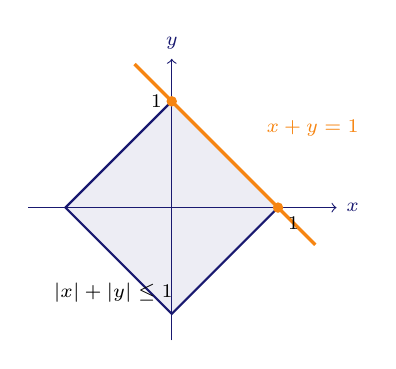
\begin{tikzpicture}[scale=1.35,every node/.style={font=\scriptsize}]
\fill[MidnightBlue!8] (1,0)--(0,1)--(-1,0)--(0,-1)--cycle;
\draw[->,MidnightBlue] (-1.35,0)--(1.55,0) node[right] {$x$};
\draw[->,MidnightBlue] (0,-1.25)--(0,1.4) node[above] {$y$};
\draw[MidnightBlue,thick] (1,0)--(0,1)--(-1,0)--(0,-1)--cycle;
\draw[BurntOrange,very thick] (-0.35,1.35)--(1.35,-0.35);
\node[BurntOrange,anchor=west] at (0.8,0.75) {$x+y=1$};
\fill[BurntOrange] (1,0) circle (1.4pt);
\fill[BurntOrange] (0,1) circle (1.4pt);
\node[below right] at (1,0) {$1$};
\node[left] at (0,1) {$1$};
\node at (-0.55,-0.8) {$|x|+|y|\le1$};
\end{tikzpicture}
